\documentclass{paper}
\usepackage[margin=3.5cm]{geometry}
\usepackage[spanish]{babel}

\title{Notas de PLS}


\usepackage{Sweave}
\begin{document}
\Sconcordance{concordance:notas_PLS.tex:notas_PLS.Rnw:%
1 7 1 1 0 16 1 1 2 4 0 2 2 4 0 1 2 3 1 1 2 4 0 2 2 12 0 1 2 86 1 1 3 2 %
0 2 1 1 3 1 0 1 3 1 0 1 3 10 0 1 2 2 1 1 3 6 0 1 2 4 1 1 4 6 0 1 2 9 1 %
1 3 5 0 1 2 7 1 1 3 5 0 1 2 2 1 1 3 23 0 1 2 1 1 1 2 7 0 2 2 7 0 2 2 7 %
0 2 2 106 0 1 2 4 1 1 3 6 0 1 2 2 1 1 3 6 0 1 2 4 1 1 2 12 0 1 2 19 1}


\maketitle

\section{Introducci\'on}

Estas notas forman parte de un Seminario de Investigaci\'on en PLS y est\'an basadas en el manual \texttt{PLS Path Modeling with R} de Gaston Sanchez. Este seminario se lleva a cabo en la Universidad Panamericana Campus Guadalajara. 

PLS-PM (Partial Least Squares Path Modeling) cuenta con las siguientes posibles definiciones:
\begin{itemize}
  \item es el enfoque de PLS al modelamiento de equaciones estructurales
  \item es un m\'etodo estad\'istico para estudiar complejas relaciones multivariadas existentes entre variables observadas y latentes
  \item es un enfoque de an\'alisis de datos para estudiar un conjunto de bloques de variables observadas donde cada bloque puede definirse por una variable latente y la relaci\'on lineal que existe entre las variables latentes.
\end{itemize}

Utilizaremos el paquete \texttt{plspm} para \texttt{R}, el cual puede instalarse como sigue
\begin{Schunk}
\begin{Sinput}
> install.packages("plspm")
\end{Sinput}
\end{Schunk}
Una vez instalado, podemos cargar la librer\'ia
\begin{Schunk}
\begin{Sinput}
> library("plspm")
\end{Sinput}
\end{Schunk}

\section{Caso de estudio: \'Indice de \'exito}

Nuestro prop\'osito ser\'a obtener un \emph{\'indice de \'exito} usando datos del futbol Soccer espa\~nol
\begin{Schunk}
\begin{Sinput}
> data(spainfoot)
\end{Sinput}
\end{Schunk}
El archivo de datos cuenta con 14 variables medidas en 20 equipos. A continuaci\'on vemos los datos correspondientes a los 5 primeros equipos de la base de datos
\begin{Schunk}
\begin{Sinput}
> head(spainfoot, n = 5)
\end{Sinput}
\begin{Soutput}
           GSH GSA  SSH  SSA GCH GCA  CSH  CSA WMH WMA LWR LRWL  YC RC
Barcelona   61  44 0.95 0.95  14  21 0.47 0.32  14  13  10   22  76  6
RealMadrid  49  34 1.00 0.84  29  23 0.37 0.37  14  11  10   18 115  9
Sevilla     28  26 0.74 0.74  20  19 0.42 0.53  11  10   4    7 100  8
AtleMadrid  47  33 0.95 0.84  23  34 0.37 0.16  13   7   6    9 116  5
Villarreal  33  28 0.84 0.68  25  29 0.26 0.16  12   6   5   11 102  5
\end{Soutput}
\end{Schunk}
La descripci\'on de cada variable se da en la siguiente tabla.



INSERTAR TABLA AQUI

\subsection{Variables latentes y manifiestas}

Una de las aplicaciones m\'as comunes de \texttt{PLS-PM} es el c\'alculo de \'indices para cuantificar alg\'un concepto clave o noci\'on de importancia. Entre estos se incluyen {\em \'Indices de Satisfacci\'on, de Motivaci\'on, de Usabilidad y de \'Exito}, entre otros. La cuesti\'on con estos conceptos es que no se pueden medir directamente. Sin embargo, es posible usar un conjunto de preguntas que de alguna manera reflejen el \'indice deseado.

\subsubsection{Variables latentes}

Hay veces en que las variables de nuestro inter\'es, como la satisfacci\'on o el \'exito, no pueden ser observadas ni medidas directamente. A estos conceptos se les conoce como {\bf variables latentes}, o tambi\'en llamadas {\em constructos, variables hipot\'eticas, intangibles} o {\em factores}.

La parte interesante se da cuando trabajamos con conceptos te\'oricos y constructos para los cuales tendemos a a concevir relaciones causales esperadas en ellos. Por ejemplo
\begin{itemize}
  \item Un director de mercadotecnia propone una nueva pol\'itica para incrementar la {\em satisfacci\'on del cliente}.
  \item Un grupo de profesores decide crear ciertas actividades extra curriculares para mejorar el {\em desempe\~no acad\'emico} de los estudiantes.
  \item Un entrenador establece un esquema de entrenamientos para mejorar el {\em desempe\~no defensivo} de su equipo.
\end{itemize}

Dado que no hay una definici\'on formal de variables latentes, en lo siguiente las consideraremos como sigue
\begin{itemize}
  \item variables hipot\'eticas
  \item ya sea imposible o muy dif\'icil de observar o medir
  \item tomadas como variables subyacentes que ayudan a explicar la asociaci\'on entre dos o m\'as variables observadas
\end{itemize}

\subsection{Modelo juguete}

Comenzaremos con el siguiente modelo simple:

\begin{quote}
Entre mejor sea la calidad del {\bf ataque}, as\'i como la calidad de la {\bf defensa}, mayor ser\'a el {\'exito.}
\end{quote}
La teor\'ia del modelo puede ser expresada de la siguiente forma abstracta:
\begin{displaymath}
exito = f(ataque, ~defensa)
\end{displaymath}
Tambi\'en se podr\'ia explicar como combinaci\'on lineal
\begin{displaymath}
exito = b_1 ataque + b_2 defensa
\end{displaymath}

\subsection{Variables manifiestas}

Aunque la escenia de las variables latentes es que no pueden ser medidas directamente, eso no significa que no tengan sentido o sean in\'utiles. Para volverlas operativas, las variables latentes se miden indirectamente mediante variables que pueden ser observadas-medidas perfectamente. A este tipo de variables se les llama {\bf variables manifiestas}, tambi\'en conocidas como {\bf indicadores}. Asumimos que las variables manifiestas contienen informaci\'on que refleja o indica alg\'un aspecto del constructo; por lo tanto, usamos la informaci\'on contenida en los indicadores para obtener una representaci\'on aproximada de la variable latente.

\subsection{Indicadores formativos y reflexivos}

Las variables latentes pueden medirse de dos maneras:
\begin{itemize}
  \item a trav\'es de sus consecuencias o efectos que se reflejan en sus indicadores
  \item a trav\'es de diversos indidacores que se asumen como causales de las variables latentes
\end{itemize}

En el primer caso, llamado {\em manera reflexiva}, se considera que las variables manifiestas o indicadores son causadas por las variables latentes. En el segundo caso, el de {\em manera formativa}, se supone que los constructos o variables latentes est\'an formados u originados de sus indicadores.
En pocas palabras, los indicadores formativos se refieren a {\bf causas}, mientras que los indicadores reflectivos a {\bf efectos} de las variables latentes o constructos.

Por ejemplo, en nuestro modelo juguete, para medir la calidad del ataque, tenemos dos posilbes enfoques:
\begin{itemize}
  \item Preguntarnos sobre los diversos estad\'isticos que {\em reflejan} el ataque, e.g. tiros a gol, tiros de esquina, goles anotados
  \item Preguntarnos sobre posibles pr\'acticas que {\em afectan} el ataque, e.g. horas de entrenamiento, tipo de comida y n\'umero de calor\'ias en la dieta de un jugador.
\end{itemize}

\subsection{Indicadores de \'Exito, Ataque y Defensa}

Hemos propuesto un modelo en el que el \'Exito depende tanto de la calidad del Ataque como de la Defensa. Estas son nuestras tres variables latentes. Ahora necesitamos construir indicadores para cada uno de estos cosntructos.

\subsection{Modelo de Trayectorias}

Un diagrama de trayectorias es una representaci\'on gr\'fica de las relaciones existentes entre constructos e indicadores. Tomaremos en cuenta la siguiente convenci\'on:
\begin{enumerate}
  \item las variables manifiestas se representan de forma rectangular
  \item las variables latentes se representan de forma el\'iptica
  \item las relaciones entre las distintas variables se representan a trav\'es de flechas
\end{enumerate}

\subsubsection{Modelo interior y exterior}

Un modelo de trayectorias completo se compone de dos submodelos: el modelo estructural, tambi'en conocido como {\bf modelo interior} y el modelo de mediciones, o {\bf modelo exterior}.

\subsubsection{Matriz del modelo interior}

Un modelo interior puede ser pensado como una red y entonces ser expresado de forma matricial, con la ayuda de \texttt{inner\_matrix}, la cual es una {\em matriz diagonal inferior booleana}, i.e. una matriz cuadrada cuyos elementos en la diagonal y arriba son cero, y los elementos bajo la diagonal son ceros o unos.

A continuaci\'on definimos la matrix interior:
\begin{Schunk}
\begin{Sinput}
> # rows of the inner model matrix
> Attack = c(0, 0, 0)
> Defense = c(0, 0, 0)
> Success = c(1, 1, 0)
> # matrix created by row binding
> foot_inner = rbind(Attack, Defense, Success)
> # add column names (optional)
> colnames(foot_inner) = rownames(foot_inner)
> # la matriz es
> foot_inner
\end{Sinput}
\begin{Soutput}
        Attack Defense Success
Attack       0       0       0
Defense      0       0       0
Success      1       1       0
\end{Soutput}
\end{Schunk}

Ahora graficamos el modelo interior
\begin{center}
\begin{Schunk}
\begin{Sinput}
> # plot the inner matrix
> innerplot(foot_inner)
\end{Sinput}
\end{Schunk}
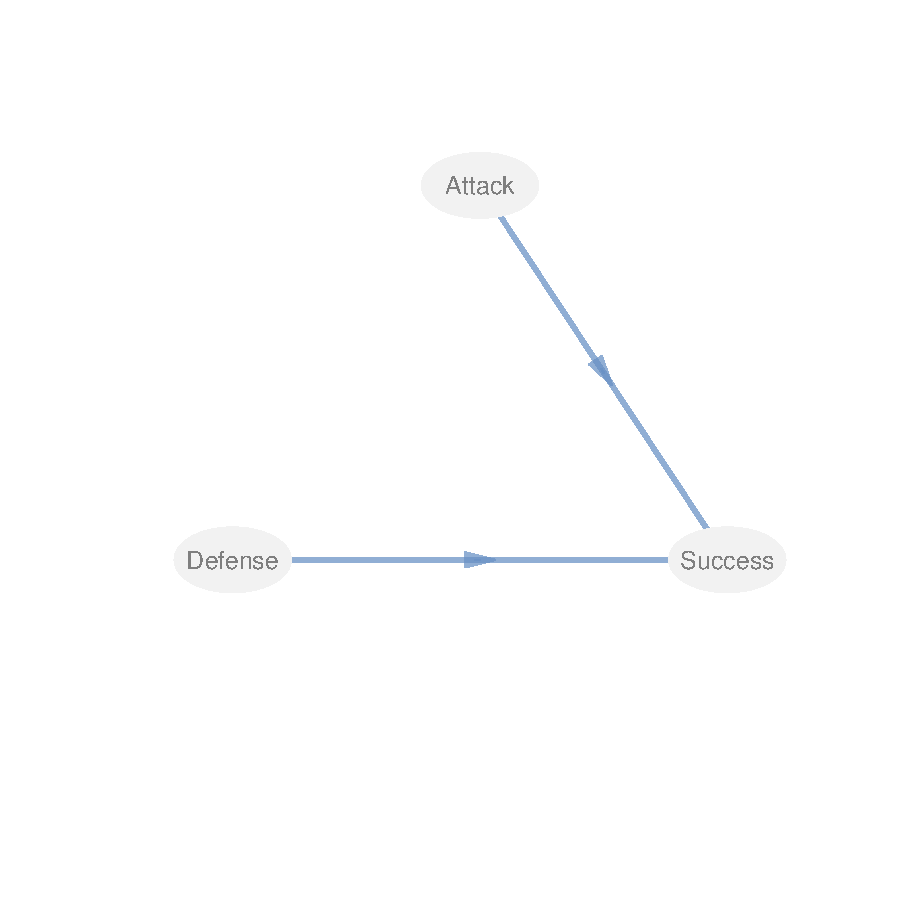
\includegraphics{notas_PLS-006}
\end{center}

\subsubsection{Lista de modelo exterior}

El modelo exterior se define utilizando una lista y un vector.
\begin{Schunk}
\begin{Sinput}
> # define list of indicators: what variables are associated with
> # what latent variables
> foot_outer = list(1:4, 5:8, 9:12)
\end{Sinput}
\end{Schunk}
La lista de arriba contiene 3 elementos, uno para cada variable latente. Cada elemento es un vector de \'indices. Entonces, la primer variable latente, Ataque, se ha asociado con las primeras cuatro columnas de nuestro conjunto de datos; la defensa est\'a asociada a las columnas 5 a 8, mientras que el \'Exito con las 9 a 12.

\subsubsection{Vector de modos}

Se definen dos modos:
\begin{enumerate}
  \item Modo {\em A}: reflectivo
  \item Modo {\em B}: formativo
\end{enumerate}

\begin{Schunk}
\begin{Sinput}
> # all latent variables are measured in a reflective way
> foot_modes = c("A", "A", "A")
\end{Sinput}
\end{Schunk}

\subsection{An\'alisis \texttt{plspm()}}

Ahora que tenemos todos los ingredientes necesarios, podemos correr nuestro primer modelo PLS-PM. La funci\'on est\'a definida como
\begin{displaymath}
plspm(Data,~inner\_ matrix, outer \_ list, modes).
\end{displaymath}
Para nuestro modelo juguete tenemos
\begin{Schunk}
\begin{Sinput}
> # run plspm analysis
> foot_pls = plspm(spainfoot, foot_inner, foot_outer, foot_modes)
\end{Sinput}
\end{Schunk}

\paragraph{Resultados de \texttt{plspm()}}

\begin{Schunk}
\begin{Sinput}
> # what's in foot_pls? foot_pls
> foot_pls
\end{Sinput}
\begin{Soutput}
Partial Least Squares Path Modeling (PLS-PM) 
---------------------------------------------
   NAME             DESCRIPTION
1  $outer_model     outer model
2  $inner_model     inner model
3  $path_coefs      path coefficients matrix
4  $scores          latent variable scores
5  $crossloadings   cross-loadings
6  $inner_summary   summary inner model
7  $effects         total effects
8  $unidim          unidimensionality
9  $gof             goodness-of-fit
10 $boot            bootstrap results
11 $data            data matrix
---------------------------------------------
You can also use the function 'summary' 
\end{Soutput}
\end{Schunk}

Para ver los coeficientes de las trayectorias
\begin{Schunk}
\begin{Sinput}
> foot_pls$path.coefs
\end{Sinput}
\begin{Soutput}
NULL
\end{Soutput}
\end{Schunk}
Consultar el modelo interior
\begin{Schunk}
\begin{Sinput}
> foot_pls$inner.mod
\end{Sinput}
\begin{Soutput}
NULL
\end{Soutput}
\end{Schunk}
Consultar el sumario del modelo interior
\begin{Schunk}
\begin{Sinput}
> foot_pls$inner.sum
\end{Sinput}
\begin{Soutput}
NULL
\end{Soutput}
\end{Schunk}
O resultados resumidos de todo
\begin{Schunk}
\begin{Sinput}
> summary(foot_pls)
\end{Sinput}
\begin{Soutput}
PARTIAL LEAST SQUARES PATH MODELING (PLS-PM) 

---------------------------------------------------------- 
MODEL SPECIFICATION 
1   Number of Cases      20 
2   Latent Variables     3 
3   Manifest Variables   12 
4   Scale of Data        Standardized Data 
5   Non-Metric PLS       FALSE 
6   Weighting Scheme     centroid 
7   Tolerance Crit       1e-06 
8   Max Num Iters        100 
9   Convergence Iters    5 
10  Bootstrapping        FALSE 
11  Bootstrap samples    NULL 

---------------------------------------------------------- 
BLOCKS DEFINITION 
      Block         Type   Size   Mode
1    Attack    Exogenous      4      A
2   Defense    Exogenous      4      A
3   Success   Endogenous      4      A

---------------------------------------------------------- 
BLOCKS UNIDIMENSIONALITY 
         Mode  MVs  C.alpha  DG.rho  eig.1st  eig.2nd
Attack      A    4    0.891   0.925     3.02    0.792
Defense     A    4    0.000   0.026     2.39    1.175
Success     A    4    0.917   0.942     3.22    0.537

---------------------------------------------------------- 
OUTER MODEL 
          weight  loading  communality  redundancy
Attack                                            
  1 GSH    0.337    0.938        0.880       0.000
  1 GSA    0.282    0.862        0.743       0.000
  1 SSH    0.289    0.841        0.707       0.000
  1 SSA    0.240    0.826        0.683       0.000
Defense                                           
  2 GCH   -0.109    0.484        0.234       0.000
  2 GCA   -0.391    0.876        0.767       0.000
  2 CSH    0.327   -0.746        0.557       0.000
  2 CSA    0.404   -0.893        0.797       0.000
Success                                           
  3 WMH    0.231    0.776        0.601       0.515
  3 WMA    0.303    0.886        0.786       0.672
  3 LWR    0.282    0.969        0.938       0.803
  3 LRWL   0.296    0.944        0.891       0.762

---------------------------------------------------------- 
CROSSLOADINGS 
          Attack  Defense  Success
Attack                            
  1 GSH    0.938   -0.516    0.898
  1 GSA    0.862   -0.339    0.752
  1 SSH    0.841   -0.414    0.771
  1 SSA    0.826   -0.336    0.639
Defense                           
  2 GCH   -0.131    0.484   -0.160
  2 GCA   -0.462    0.876   -0.575
  2 CSH    0.319   -0.746    0.481
  2 CSA    0.421   -0.893    0.593
Success                           
  3 WMH    0.709   -0.423    0.776
  3 WMA    0.773   -0.711    0.886
  3 LWR    0.844   -0.538    0.969
  3 LRWL   0.860   -0.589    0.944

---------------------------------------------------------- 
INNER MODEL 
$Success
             Estimate   Std. Error     t value   Pr(>|t|)
Intercept   -2.00e-16       0.0922   -2.17e-15   1.00e+00
Attack       7.57e-01       0.1044    7.25e+00   1.35e-06
Defense     -2.84e-01       0.1044   -2.72e+00   1.47e-02

---------------------------------------------------------- 
CORRELATIONS BETWEEN LVs 
         Attack  Defense  Success
Attack     1.00   -0.470    0.890
Defense   -0.47    1.000   -0.639
Success    0.89   -0.639    1.000

---------------------------------------------------------- 
SUMMARY INNER MODEL 
               Type     R2  Block_Communality  Mean_Redundancy    AVE
Attack    Exogenous  0.000              0.753            0.000  0.753
Defense   Exogenous  0.000              0.589            0.000  0.589
Success  Endogenous  0.856              0.804            0.688  0.804

---------------------------------------------------------- 
GOODNESS-OF-FIT 
[1]  0.7823

---------------------------------------------------------- 
TOTAL EFFECTS 
        relationships  direct  indirect   total
1   Attack -> Defense   0.000         0   0.000
2   Attack -> Success   0.757         0   0.757
3  Defense -> Success  -0.284         0  -0.284
\end{Soutput}
\end{Schunk}

\paragraph{Visualizando los resultados}

Veamos los resultados del modelo interior
\begin{center}
\begin{Schunk}
\begin{Sinput}
> # plotting results (inner model)
> plot(foot_pls)
\end{Sinput}
\end{Schunk}
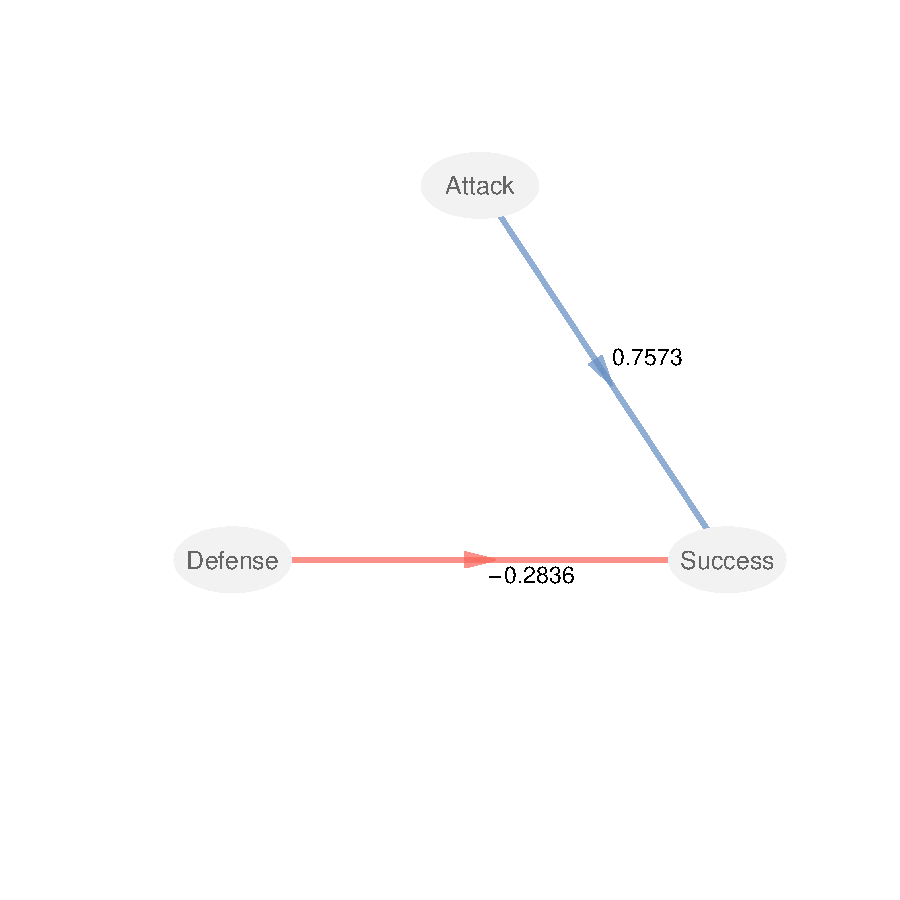
\includegraphics{notas_PLS-015}
\end{center}

\begin{center}
\begin{Schunk}
\begin{Sinput}
> # plotting loadings of the outer model
> plot(foot_pls, what = "loadings", arr.width = 0.1)
\end{Sinput}
\end{Schunk}
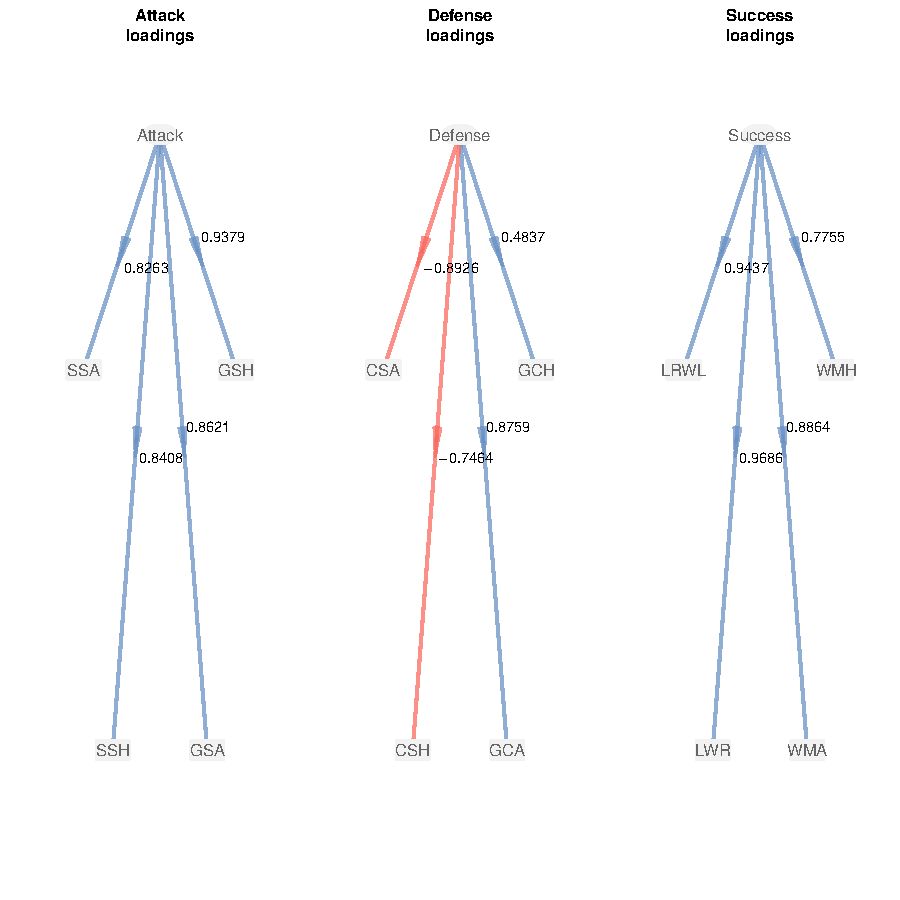
\includegraphics{notas_PLS-016}
\end{center}

\paragraph{Mu\'estrame el \'Indice}

Veamos el \'indice de los 5 primeros equipos
\begin{Schunk}
\begin{Sinput}
> head(foot_pls$scores, n = 5)
\end{Sinput}
\begin{Soutput}
               Attack     Defense   Success
Barcelona   2.6115644 -1.74308968 2.7891432
RealMadrid  1.7731019 -1.13283765 2.3245911
Sevilla    -0.1123198 -2.24651002 0.5540990
AtleMadrid  1.5333996  0.02391761 0.7770707
Villarreal  0.2801361  0.16761000 0.6084217
\end{Soutput}
\end{Schunk}

Sin embargo, todav\'ia hay que hacer ajustes al modelo.

















\end{document}
